\documentclass[a4paper]{article}

% Language and font encodings
\usepackage[english]{babel}
\usepackage{amsmath}
\usepackage{graphicx}
\usepackage{tabularx}
\usepackage{natbib}
\usepackage[colorinlistoftodos]{todonotes}
\usepackage[colorlinks=true, allcolors=blue]{hyperref}
\usepackage{wrapfig}
\DeclareMathAlphabet{\pazocal}{OMS}{zplm}{m}{n}
\usepackage{setspace}
\usepackage{hyperref}
\hypersetup{
    colorlinks=true,
    linkcolor=blue,
    filecolor=magenta,      
    urlcolor=cyan,
}
\urlstyle{same}

%%%%%%%%%%%%%%%%%%%%%%%%%%%%%%%%%%%%%%%%%%%%%%%%%%%%%%%%%%%%%%%%%%%%%%%%%%%%%%%%

\begin{document}

\begin{center}
  {\Large \bf Milestone 1: The background evolution of the universe.}\\[4ex]
  {\large Daniel Herman}\\[4ex]
  \normalsize
  \today
  \vspace*{2ex}
      
  \begin{minipage}[t]{15cm}
      
  {\bf Abstract. }The background cosmology of the universe was simulated numerically.
	
  \vspace*{2ex}
  \end{minipage}

\end{center}

%%%%%%%%%%%%%%%%%%%%%%%%%%%%%%%%%%%%%%%%%%%%%%%%%%%%%%%%%%%%%%%%%%%%%%%%%%%%%%%%

\section{Introduction}\label{sec:intro}

This report focuses on Milestone 1 of the semester long project. This is the first step towards simulating the Cosmic Microwave Background. Milestone 1 is aimed at simulating the expansion of the universe, as well as the evolution of densities. I have used a general case, which includes the neutrino density. In this report, we look at the evolution of the Hubble parameter, characteristic densities, and the conformal time as the universe ages.\\

A skeleton code was provided to assist in creation of the code. Additional FORTRAN code was also provided to expedite the development, including a parameter file and an ODE solver.\\

The calculation portion of Milestone 1 was written in FORTRAN 90, and the plotting was done using Python. The code can be found at \url{https://github.com/hermda02/CosmologyII}.

%%%%%%%%%%%%%%%%%%%%%%%%%%%%%%%%%%%%%%%%%%%%%%%%%%%%%%%%%%%%%%%%%%%%%%%%%%%%%%%%

\section{Equations}\label{sec:equa}

For this portion of the project we assume a flat universe, and so we use the Friedmann-Robertson-Walker metric. This metric gives us the line element.

\begin{align}\label{FRW}
ds^2 &= -dt^2 + a^2(t)d\vec{y}^2\\
     &= a^2(\eta)[-d{\eta}^2 + d\vec{y}^2]
\end{align}
where $a(t)$ is the scale factor, $\eta$ is the conformal time, and $\vec{y}$ is the vector describing the spatial portion of the line element.\\

The scale factor $a$ corresponds to the redshift $z$ in the following way

\begin{align}
a(t) = \dfrac{a_0}{1+z} \Rightarrow z = \dfrac{a_0}{a} -1
\end{align}

Another parameter $x$ is also introduced here.
\begin{align}
x = \ln(a)
\end{align}

In our model, we assume that the universe is composed of baryons (b), Cold Dark Matter (CDM, m), radiation (r), neutrinos ($\nu$), and dark energy ($\Lambda$). We utilize the Friedmann equation to describe the evolution of the Hubble parameter, $H$, over time with respect to the above quantities

\begin{equation}\label{Hubble}
H = \dfrac{\dot{a}}{a} = H_0\sqrt{(\Omega_b + \Omega_m)a^{-3} + (\Omega_r + \Omega_{\nu})a^{-4} + \Omega_{\Lambda}}
\end{equation}
where the dot above the $a$ represents the first time derivative. A scaled Hubble constant $\pazocal{H}$ is also introduced, purely for convenience, where $\pazocal{H} \equiv aH$. \\


The Friedmann equations also describe how each component evolves with time

\begin{equation} \label{eq:rho}
\begin{aligned}
\rho_m =& \rho_{m,0}a^{-3}\\
\rho_b =& \rho_{b,0}a^{-3}\\
\rho_r =& \rho_{r,0}a^{-4}\\
\rho_{\nu} =& \rho_{\nu,0}a^{-4}\\
\rho_{\Lambda} =& \rho_{\Lambda,0}
\end{aligned}
\end{equation}

We will also need to calculate the size of the particle horizon as a function of time. We note that

\begin{equation*}
\dfrac{d\eta}{dt} = \dfrac{c}{a}
\end{equation*} 
which can be rewritten as
\begin{equation}\label{eta}
\dfrac{d\eta}{da} = \dfrac{c}{a \pazocal{H}}
\end{equation}
Solving for $\eta$ numerically can be done either through direct integration or by using an ODE solver. Since an ODE solver is included in the provided code, we utilize this method.

\clearpage

%%%%%%%%%%%%%%%%%%%%%%%%%%%%%%%%%%%%%%%%%%%%%%%%%%%%%%%%%%%%%%%%%%%%%%%%%%%%%%%%

\section{Implementation}\label{sec:Imp}
The skeleton code provided is written using FORTRAN90, which is commonly used by astronomers. Code for this milestone was all written in FORTRAN90, except for the plotting of the results which is done using Python.\\

Arrays are allocated for $a$, $x$, $z$, and $\eta$, as well as all of the $\Omega$ and $\rho$ values. An array is also created for the $H$ values as well. We will look at the behavior of each of these quantities as a function of time.\\

We initialize $a$, which represents the scale factor by setting $a_{rec} = 10^{-10}$ and $a_0 = 1$ (today). These values are used to determine the values of $x$. The rest of the array for $x$ is filled in a linear fashion, using 1000 equally spaced steps. The resulting values of $x$ are used to solve for the values of the $a$ and $z$ arrays, each with 1000 points.\\

With our values of $a$ calculated between recombination and today, we can solve for $H$, $\pazocal{H}$, and the densities $\rho_x$ and $\Omega_x$ as a function of time using \ref{Hubble} and \ref{eq:rho}. Functions to solve for $H$, $\pazocal{H}$ and $\eta$ were created so that these could easily be called multiple times throughout the code.\\

We then solve for the values of $\eta$. As mentioned above, we utilize the provided FORTRAN90 ODE solver on the equation \ref{eta}. In order to solve this ODE, we must provide an initial value to $\eta$. This can be found considering the fact that radiation density dominates in the early universe, as $a \rightarrow 0$.
Explicitly, this shows that

\begin{equation}\label{eq:etainit}
\eta(a) = \dfrac{a}{H_0\sqrt{\Omega_r + \Omega_{\nu}}}
\end{equation}
for small values of $a$. We use the inital value of $a = 10^{-10}$ to initialize the ODE solver. This is used to solve the integral

\begin{equation}\label{eq:etaint}
\eta(a) = \int_0^a \dfrac{c da'}{a' \pazocal{H}}
\end{equation}

These values are plugged into the ODE solver to return $\eta(x)$. An included spline program is also utilized to resolve the values of $\eta$ in between the calculated grid points, which will be useful in future calculations for this project. 

\clearpage

%%%%%%%%%%%%%%%%%%%%%%%%%%%%%%%%%%%%%%%%%%%%%%%%%%%%%%%%%%%%%%%%%%%%%%%%%%%%%%%%

\section{Results}\label{Results}

We see in figure \ref{fig:dens} that in the early universe, the radiation density dominates in comparison to the other contributions ot the overall density. As we approach lower redshift, we see the dark matter and baryon densities begin to increase.
\begin{wrapfigure}{i}{0.65\textwidth}\label{fig:dens}
  \begin{center}
    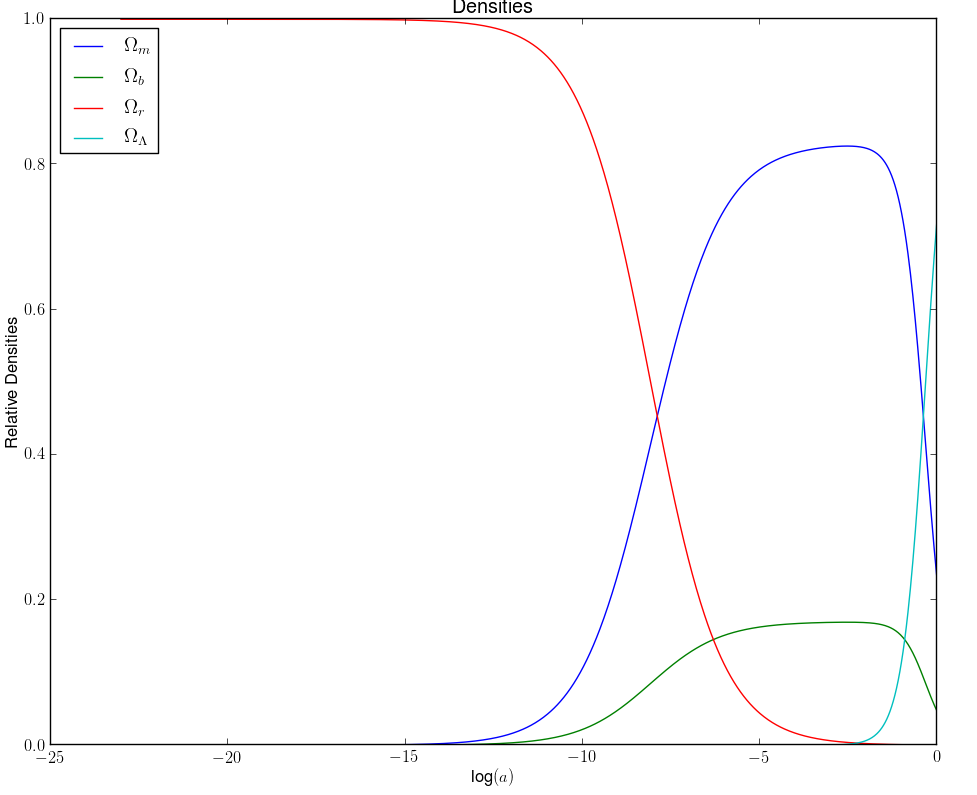
\includegraphics[width=0.65\textwidth]{densities2}
  \end{center}
  \caption{The evolution of $\Omega$s as a function of $x$.}
\end{wrapfigure} 
As expected, the dark matter and baryonic matter contributions behave in the same fashion. For very low redshift, the matter densities taper off quickly and the vacuum energy $\Omega_{\Lambda}$ quickly becomes the most dominant factor contributing to the Hubble parameter.

In figure \ref{fig:etax} we use $\log(\eta)$ to better observe the evolution of the conformal time $\eta(x)$. The conformal time measures the size of the particle horizon, which quickly expands and approaches $10^4$ Mpc.\\

The current measured particle horizon (size of the observable universe) is roughly 14Gpc, so our simulation appears to be working properly. We see 



\begin{figure}[hb!]\label{fig:etax}
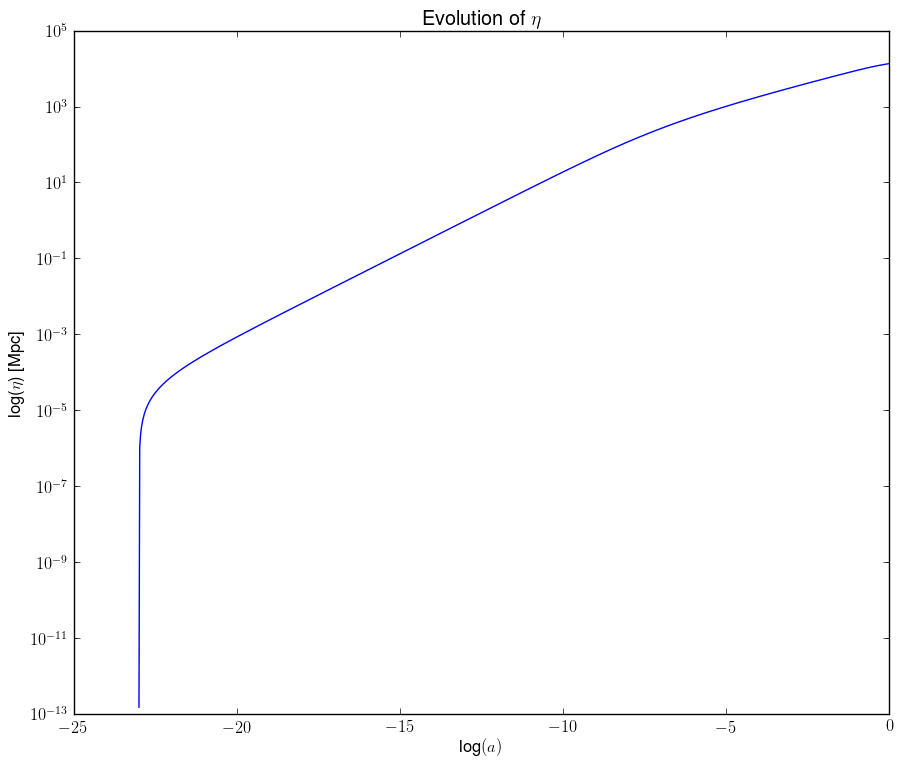
\includegraphics[scale=0.25]{eta_x2}
\caption{The evolution of $\eta$ as a function of $x = \ln(a)$.}
\end{figure}

\clearpage

The Hubble parameter $H$ is plotted in figures \ref{fig:hx} and \ref{fig:hz} as functions of $x$ and $z$ respectively. I cannot speak to the validity of the evolution of $H$, however we do see that $H \rightarrow H_0$ as $z \rightarrow 0$. 
\begin{center}
\begin{figure}[ht!]\label{fig:hx}
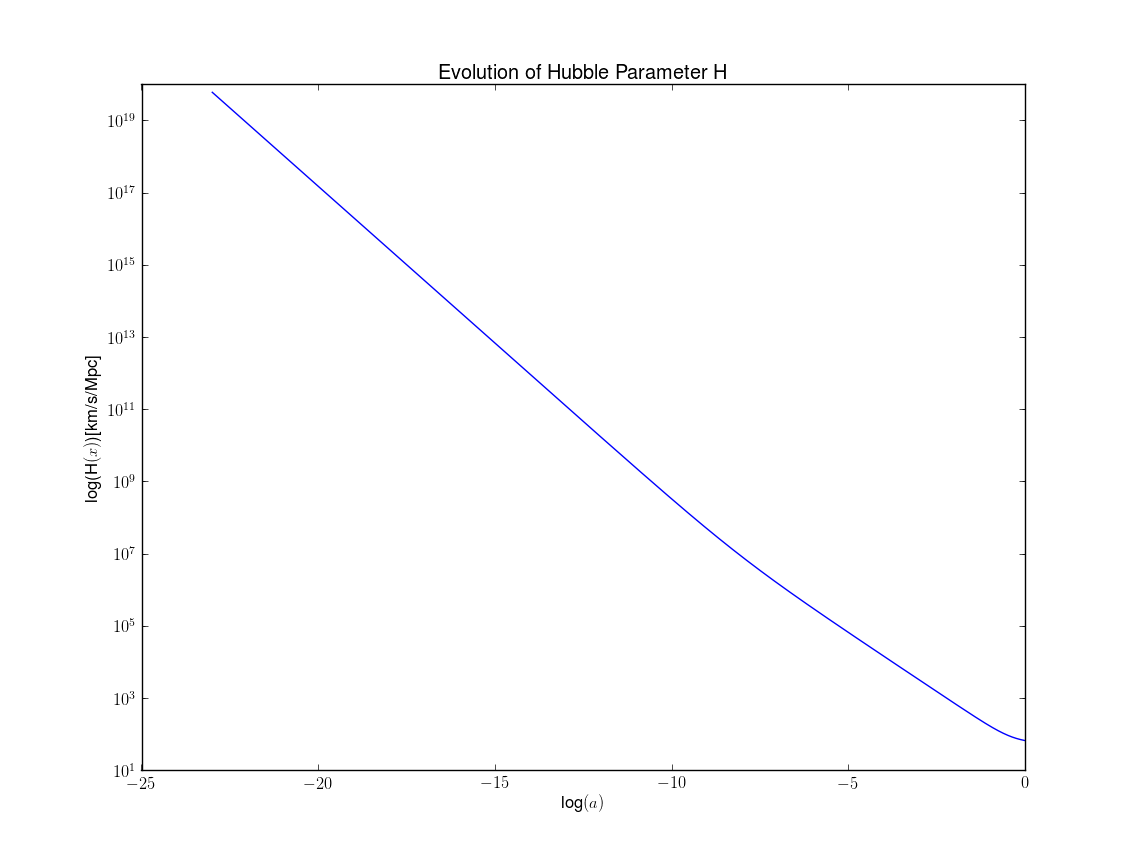
\includegraphics[scale=0.35]{hx}
\caption{The evolution of the Hubble parameter as a function of $x$. $\ln(H)$ is used on the y-axis for clarity.}
\end{figure}

\begin{figure}[h!]\label{fig:hz}
\centering
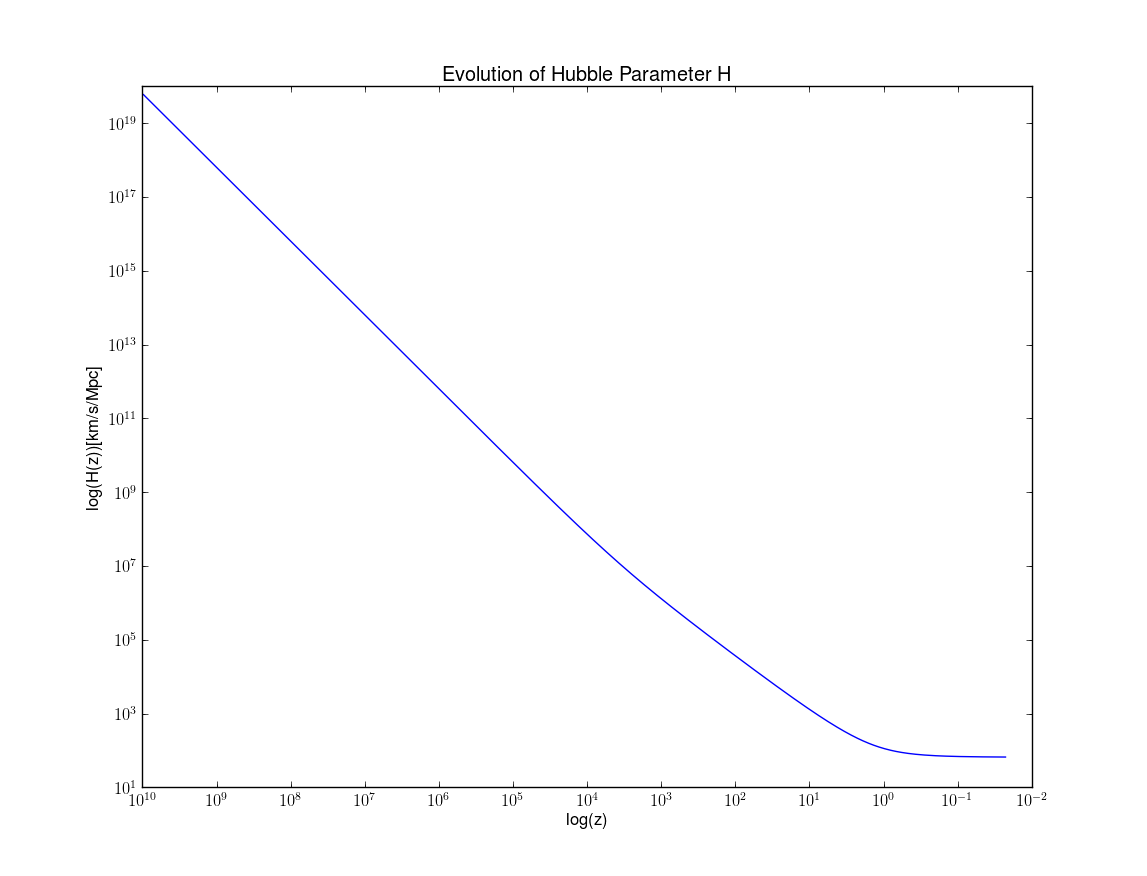
\includegraphics[scale=0.35]{hz}
\caption{The evolution of the Hubble parameter as a function of redshift. A log-log plot is used to easily observe the behavior.}
\end{figure}
\end{center}

%%%%%%%%%%%%%%%%%%%%%%%%%%%%%%%%%%%%%%%%%%%%%%%%%%%%%%%%%%%%%%%%%%%%%%%%%%%%%%%%

\section{Conclusion}\label{sec:conc}
All of the calculations required for Milestone 1 were completed and produced the expected results. The integration of the ODE solver and the spline technique have worked as expected as well. The code is now prepared for further work on the project as a whole.

%%%%%%%%%%%%%%%%%%%%%%%%%%%%%%%%%%%%%%%%%%%%%%%%%%%%%%%%%%%%%%%%%%%%%%%%%%%%%%%%




\end{document}